\documentclass[11pt,a4paper]{article}
\usepackage[utf8]{inputenc}
\usepackage[T1]{fontenc}
% babel portugues se existir (Overleaf); localmente cai para o default se faltar texlive-langportuguese
\IfFileExists{portuguese.ldf}{\usepackage[portuguese]{babel}}{}
\usepackage[margin=2.4cm]{geometry}
\usepackage{lmodern}
\usepackage{amsmath}
\usepackage{booktabs}
\usepackage{xcolor}
\usepackage{listings}
\usepackage{tikz}
\usetikzlibrary{arrows.meta,positioning,fit}
\usepackage[colorlinks=true,linkcolor=blue!50!black,urlcolor=blue!50!black]{hyperref}

\newcommand{\code}[1]{\texttt{\detokenize{#1}}}

\lstset{
  basicstyle=\ttfamily\footnotesize,
  keywordstyle=\color{blue!60!black}\bfseries,
  commentstyle=\color{gray},
  stringstyle=\color{red!50!black},
  language=Python,
  columns=fullflexible,
  keepspaces=true,
  frame=single,
  rulecolor=\color{black!25},
  breaklines=true,
  showstringspaces=false,
  xleftmargin=0.5em,
  xrightmargin=0.5em
}

\title{Integra\c{c}\~ao ACN-Sim e pandapower em malha fechada}
\author{Guia de trabalho para a tese}
\date{}

\begin{document}
\maketitle

\section{Resumo}

\begin{itemize}
  \item A documenta\c{c}\~ao do ACN-Sim descreve a liga\c{c}\~ao ao pandapower como \emph{sequencial}: a sa\'ida do ACN-Sim \'e a entrada do simulador de rede.
  \item O feedback da rede para o ACN-Sim est\'a indicado como trabalho futuro.
  \item O pacote \code{acnportal} 0.3.3 instalado n\~ao cont\'em c\'odigo de rede. O c\'odigo de integra\c{c}\~ao est\'a num reposit\'orio \`a parte, \code{caltech-netlab/acnportal-experiments}.
  \item Logo, a co-simula\c{c}\~ao em malha fechada tem de ser constru\'ida por n\'os. Isso \'e ao mesmo tempo um risco e uma contribui\c{c}\~ao da tese.
  \item A boa not\'icia \'e que a API do ACN-Sim tem os pontos de acoplamento certos. Validei um prot\'otipo descart\'avel (n\~ao \'e o esqueleto do projeto) em que o escalonador l\^e a tens\~ao medida no pandapower no per\'iodo anterior. Um dia de 288 passos de 5 minutos corre em cerca de 4 segundos.
\end{itemize}

\paragraph{Fontes.}
O paper ACN-Sim (arXiv 2012.02809), a sec\c{c}\~ao de co-simula\c{c}\~ao com simuladores de rede, e o c\'odigo-fonte do \code{acnportal} 0.3.3.
A pesquisa na web indicou o reposit\'orio \code{acnportal-experiments} como local dos exemplos com pandapower e OpenDSS, tamb\'em com acoplamento unidirecional.
N\~ao abri esse reposit\'orio nem a documenta\c{c}\~ao em \code{acnportal.readthedocs.io}, por isso conv\'em confirm\'a-los antes de assumir que n\~ao h\'a nada reutiliz\'avel.

\section{Pontos de acoplamento na API do ACN-Sim}

\begin{center}
\footnotesize
\begin{tabular}{@{}p{7.7cm}p{8.1cm}@{}}
\toprule
Elemento & Para que serve na co-simula\c{c}\~ao \\
\midrule
\code{Simulator(network, scheduler, events, start, period)} & Ciclo principal. \code{period} \'e em minutos. \\
\code{BaseAlgorithm.schedule(active_sessions)} & Aqui vive o MPC. Devolve um dicion\'ario de esta\c{c}\~ao para lista de correntes (A). \\
\code{scheduler.max_recompute = 1} & For\c{c}a a chamada do escalonador em todos os per\'iodos. Sem isto, s\'o \'e chamado quando h\'a eventos. \\
\code{interface.current_time} & \'Indice do per\'iodo atual. \\
\code{interface.last_actual_charging_rate} & Correntes (A) do per\'iodo anterior, indexadas por \emph{session id}. \\
\code{interface.evse_voltage(id)}, \code{evse_phase(id)} & Tens\~ao e \^angulo de fase de cada EVSE. \\
\code{interface.max_pilot_signal(id)} & Corrente m\'axima do EVSE. \\
\code{interface.remaining_amp_periods(s)} & Energia que falta, em A$\cdot$per\'iodos. \\
\code{interface.get_constraints()} & Matriz de restri\c{c}\~oes de corrente da rede de carregamento. \\
\code{sim.charging_rates} & Matriz esta\c{c}\~oes $\times$ tempo com as correntes reais (A). \\
\code{Linear2StageBattery(cap, init, max_power)} & Bateria do EV, em kWh e kW. \\
\bottomrule
\end{tabular}
\end{center}

Convers\~ao de unidades, igual \`a usada internamente por \code{remaining_amp_periods}:
\[
P_{\mathrm{kW}} = \frac{I_{\mathrm{A}}\, V_{\mathrm{EVSE}}}{1000},
\qquad
\text{A}\cdot\text{per\'iodos} = \frac{E_{\mathrm{kWh}} \cdot 1000}{V_{\mathrm{EVSE}}}\cdot\frac{60}{\text{period}}.
\]

\paragraph{O que o ACN-Sim n\~ao tem.}
O modelo \code{Battery} do ACN-Sim \'e o da bateria do EV.
N\~ao h\'a bateria estacion\'aria, PV nem carga de edif\'icio.
Tudo isso entra como s\'eries externas e como modelos nossos, tanto no MPC como na ``planta''.

\section{Arquitetura em malha fechada}

\begin{center}
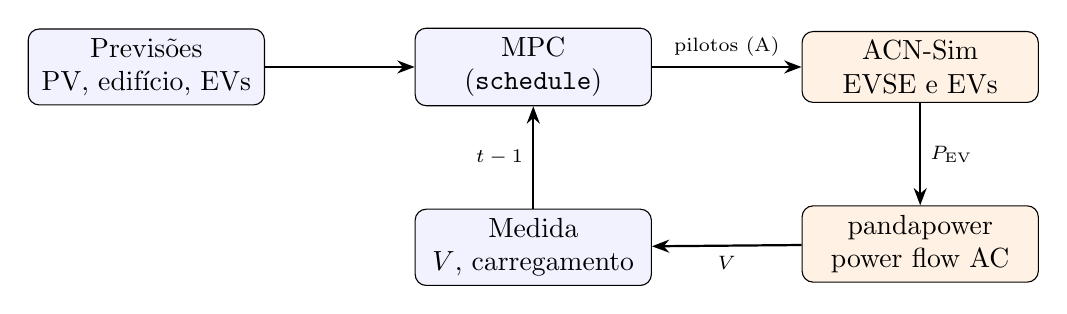
\begin{tikzpicture}[
  node distance=1.3cm and 1.9cm,
  box/.style={draw, rounded corners, minimum width=3.0cm, minimum height=0.9cm, align=center, fill=blue!5},
  plant/.style={draw, rounded corners, minimum width=3.0cm, minimum height=0.9cm, align=center, fill=orange!10},
  arr/.style={-{Stealth[length=2.2mm]}, thick}
]
  \node[box] (fc) {Previs\~oes\\PV, edif\'icio, EVs};
  \node[box, right=of fc] (mpc) {MPC\\(\code{schedule})};
  \node[plant, right=of mpc] (acn) {ACN-Sim\\EVSE e EVs};
  \node[plant, below=of acn] (pf) {pandapower\\power flow AC};
  \node[box, below=of mpc] (meas) {Medida\\$V$, carregamento};
  \draw[arr] (fc) -- (mpc);
  \draw[arr] (mpc) -- node[above, font=\scriptsize]{pilotos (A)} (acn);
  \draw[arr] (acn) -- node[right, font=\scriptsize]{$P_{\mathrm{EV}}$} (pf);
  \draw[arr] (pf) -- node[below, font=\scriptsize]{$V$} (meas);
  \draw[arr] (meas) -- node[left, font=\scriptsize]{$t-1$} (mpc);
\end{tikzpicture}
\end{center}

\paragraph{Atraso de um per\'iodo.}
O escalonador \'e chamado no in\'icio do per\'iodo $t$ e s\'o v\^e o que se passou at\'e $t-1$.
Isto \'e realista (lat\^encia de medida) e liga-se \`a ideia de tratar atrasos como erro de modelo no paper de Pajic et al.

\paragraph{Duas formas de ligar o power flow.}
\begin{enumerate}
  \item \textbf{Dentro do escalonador.} Mais simples, mas \code{last_actual_charging_rate} s\'o inclui as sess\~oes ainda ligadas no per\'iodo $t$. Uma sess\~ao que terminou exatamente em $t$ fica de fora e a carga \'e subestimada.
  \item \textbf{Numa subclasse de \code{Simulator}} (recomendada). Sobrep\~oe-se \code{_store_actual_charging_rates}, que o ciclo chama logo ap\'os aplicar os pilotos. A\'i usa-se a matriz \code{charging_rates} completa, sem perder sess\~oes.
\end{enumerate}

Testei a segunda: a tens\~ao m\'inima do dia coincide exatamente (diferen\c{c}a m\'axima de 0) com a obtida a repetir o power flow a posteriori sobre \code{sim.charging_rates}.

\begin{lstlisting}
class CoSimulator(acnsim.Simulator):
    def __init__(self, *args, grid, **kwargs):
        super().__init__(*args, **kwargs)
        self.grid, self.v_site = grid, 1.0

    def _store_actual_charging_rates(self):
        super()._store_actual_charging_rates()
        t = self._iteration
        kw = float(self.charging_rates[:, t].sum() * V_EVSE / 1000)
        self.v_site = self.grid.solve(t, kw)   # mesmo periodo, correntes exatas

class MPCWithGrid(BaseAlgorithm):
    def __init__(self):
        super().__init__()
        self.max_recompute = 1                 # chamar em todos os periodos

    def schedule(self, sessions):
        v_prev = self.sim.v_site               # medida do periodo t-1
        return self.mpc.solve(sessions, v_prev)  # dict {station_id: [A, ...]}
\end{lstlisting}

\section{Pitfalls que encontrei}

\begin{itemize}
  \item A rede de carregamento precisa de pelo menos uma restri\c{c}\~ao. Sem ela, o \code{Simulator} falha ao validar (\code{constraint_matrix} \'e \code{None}).
  \item O ACN-Sim e o pandapower usam conven\c{c}\~oes diferentes: correntes por esta\c{c}\~ao e fase de um lado, pot\^encia por barramento do outro. A convers\~ao deve ficar num s\'o s\'itio.
  \item A simula\c{c}\~ao termina quando a fila de eventos esvazia. No teste, o dia parou ao fim de 249 dos 288 passos. Para alinhar com s\'eries de PV e edif\'icio de 24 h, adicionar um evento final.
  \item O pacote exige \code{setuptools<81} (usa \code{pkg_resources}). J\'a est\'a fixado no ambiente.
  \item Um schedule invi\'avel levanta \code{InvalidScheduleError}. O MPC tem de respeitar as restri\c{c}\~oes que a \code{Interface} exp\~oe e os n\'iveis de piloto permitidos (por exemplo, o m\'inimo de 6 A do J1772).
  \item Cada passo custa cerca de 15 ms com o pandapower e numba, incluindo o escalonador trivial. Um MPC por cen\'arios vai dominar o tempo.
\end{itemize}

\section{Uma rede verosimil}

\subsection{O que n\~ao serve}

A rede CIGRE LV do pandapower (\code{create_cigre_network_lv}) \'e a primeira ideia, mas n\~ao serve tal como est\'a.
Com as cargas base, a tens\~ao m\'inima do alimentador comercial j\'a \'e 0{,}912~pu, \emph{sem} nenhum EV.
No prot\'otipo, um parque de 30 carregadores no barramento C9 baixou a tens\~ao m\'inima para 0{,}75~pu.
Esse valor n\~ao \'e realista e tornaria qualquer conclus\~ao sobre o MPC irrelevante.

\subsection{Proposta: rede param\'etrica pr\'opria}

Construir a rede com tipos standard do pandapower:
fronteira de m\'edia tens\~ao (20~kV, $S_{sc}=250$~MVA), transformador \code{0.63 MVA 20/0.4 kV}, cabo \code{NAYY 4x150 SE} com comprimento e n\'umero de cabos em paralelo como par\^ametros, cargas vizinhas num barramento, e o \emph{site} (edif\'icio, PV, bateria e carregadores) no fim do cabo.
Duas configura\c{c}\~oes d\~ao uma dimens\~ao experimental, a for\c{c}a da rede.

\begin{center}
\small
\textbf{Configura\c{c}\~ao A (forte):} 80~m, 3 cabos em paralelo, edif\'icio 40~kW\\[0.4em]
\begin{tabular}{@{}lcccc@{}}
\toprule
Carga EV (kW) & 0 & 120 & 220 & 300 \\
\midrule
$V$ no site (pu) & 0{,}997 & 0{,}990 & 0{,}984 & 0{,}979 \\
Transformador (\%) & 7 & 26 & 42 & 55 \\
Cabo (\%) & 7 & 29 & 47 & 62 \\
\bottomrule
\end{tabular}

\vspace{1em}

\textbf{Configura\c{c}\~ao B (fraca):} 300~m, 1 cabo, vizinhos 80~kW no barramento BT\\[0.4em]
\begin{tabular}{@{}lcccc@{}}
\toprule
Carga EV (kW) & 0 & 40 & 80 & 120 \\
\midrule
$V$ no site (pu) & 0{,}976 & 0{,}959 & 0{,}940 & 0{,}921 \\
Transformador (\%) & 20 & 27 & 34 & 41 \\
Cabo (\%) & 23 & 45 & 69 & 93 \\
\bottomrule
\end{tabular}
\end{center}

\paragraph{Leitura dos resultados.}
Na configura\c{c}\~ao A a tens\~ao quase n\~ao restringe: o que limita \'e o pico, o transformador e o cabo.
\'E o caso t\'ipico de um parque de trabalho com liga\c{c}\~ao dedicada.
Na B, a tens\~ao desce abaixo de 0{,}95~pu por volta dos 60~kW de EVs, e o cabo chega a 93\,\% a 120~kW.
\'E a configura\c{c}\~ao onde um controlador sens\'ivel \`a tens\~ao tem algo a mostrar.
O limite de 0{,}95~pu \'e uma escolha de projeto minha. O limite estatut\'ario habitual (EN~50160) \'e $\pm10\,\%$ e deve ser confirmado.

\paragraph{Dimensionamento do site (a calibrar).}
30 carregadores de 7{,}4~kW (222~kW), edif\'icio entre 40 e 100~kW, PV de cerca de 80~kWp, bateria de cerca de 100~kW por 200~kWh.
S\~ao n\'umeros meus, por ajustar \`a literatura (por exemplo, o sistema de Torres et al. chega a 240 EVs e carregadores) e aos dados do ACN-Data.

\subsection{Trif\'asico}

O ACN-Sim modela correntes por fase, e o pandapower consegue um power flow desequilibrado com \code{runpp_3ph} e \code{create_asymmetric_load}.
Os tipos standard n\~ao trazem dados de sequ\^encia zero. Sem eles falha logo com \code{KeyError} (por exemplo \code{x0x_max} e \code{r0_ohm_per_km}).
Foi preciso fornecer:
\begin{itemize}
  \item no \code{ext_grid}: \code{x0x_max} e \code{r0x0_max};
  \item nas linhas: \code{r0_ohm_per_km}, \code{x0_ohm_per_km} e \code{c0_nf_per_km};
  \item no transformador: \code{vk0_percent}, \code{vkr0_percent}, \code{mag0_percent}, \code{mag0_rx}, \code{si0_hv_partial} e \code{vector_group}.
\end{itemize}
Usei $r_0=4r_1$ e $x_0=3{,}5x_1$ como valores t\'ipicos assumidos.
Estes valores s\~ao um pressuposto meu e t\^em de ser validados.

Resultado no site (cabo de 300~m, sem cargas vizinhas) com cargas diferentes em cada fase A, B e C:

\begin{center}
\small
\begin{tabular}{@{}lccccc@{}}
\toprule
Carga A/B/C (kW) & Total & $V_A$ & $V_B$ & $V_C$ & Desequil\'ibrio (\%) \\
\midrule
20/20/20 & 60 & 0{,}975 & 0{,}975 & 0{,}975 & 0{,}00 \\
30/20/20 & 70 & 0{,}948 & 0{,}984 & 0{,}979 & 0{,}57 \\
45/0/0 & 45 & 0{,}876 & 1{,}043 & 1{,}020 & 2{,}51 \\
\bottomrule
\end{tabular}
\end{center}

Concentrar a carga numa fase derruba a tens\~ao dessa fase (0{,}876~pu com apenas 45~kW) e faz subir as outras duas, por deslocamento do neutro.
Isto refor\c{c}a o argumento do paper ACN-Sim sobre o equil\'ibrio de fases, e \'e um bom motivo para o MPC saber em que fase est\'a cada carregador.
Um caso mais extremo (100~kW numa s\'o fase, com cargas vizinhas desequilibradas) n\~ao convergiu.
A n\~ao-converg\^encia deve ser tratada como evento na simula\c{c}\~ao, e n\~ao como erro.

\section{O que o prot\'otipo mostrou}

O prot\'otipo descart\'avel (guardado fora do projeto) correu um dia com 30 carregadores, na rede CIGRE LV, que sabemos ser n\~ao realista.
Serve s\'o para provar a liga\c{c}\~ao.

\begin{center}
\small
\begin{tabular}{@{}lcc@{}}
\toprule
& Sem feedback & Escalonador l\^e a tens\~ao \\
\midrule
Tens\~ao m\'inima (pu) & 0{,}750 & 0{,}794 \\
Pico de carga (kW) & 175 & 161 \\
Energia entregue / pedida (kWh) & 563 / 563 & 403 / 563 \\
\bottomrule
\end{tabular}
\end{center}

O feedback tem efeito mensur\'avel no comportamento da rede e custa energia n\~ao entregue, que \'e o compromisso que o MPC vai gerir de forma otimizada.
Estes n\~ao s\~ao resultados cient\'ificos: o escalonador \'e uma heur\'istica, e a rede n\~ao \'e realista.

\section{Pr\'oximos passos}

\begin{enumerate}
  \item Abrir \code{acnportal-experiments} e a documenta\c{c}\~ao online para ver o que reutilizar (notebooks com pandapower e OpenDSS).
  \item Fixar a rede param\'etrica (configura\c{c}\~oes A e B) e validar a calibra\c{c}\~ao com o professor.
  \item Reproduzir o case study sequencial do paper com pandapower, antes de ligar o feedback.
  \item S\'o depois, o esqueleto do projeto.
\end{enumerate}

\end{document}
